\section{A conceptual framework of labour market outcomes}\label{sec:framework}
A woman's decision whether to participate or not in the labour market involves a complex set of fundamental drivers in conjunction with life-cycle circumstances, which can be broadly classified as (i) personal preferences, (ii) socio-economic constraints, and (iii) gender role conformity (Figure~\ref{fig:framework}). These three fundamental drivers are conditional on or are determined by the prevailing gender social norms in the society that a woman inhabits.

\begin{figure}[htb]
	\centering
	\caption{Conceptual framework}
	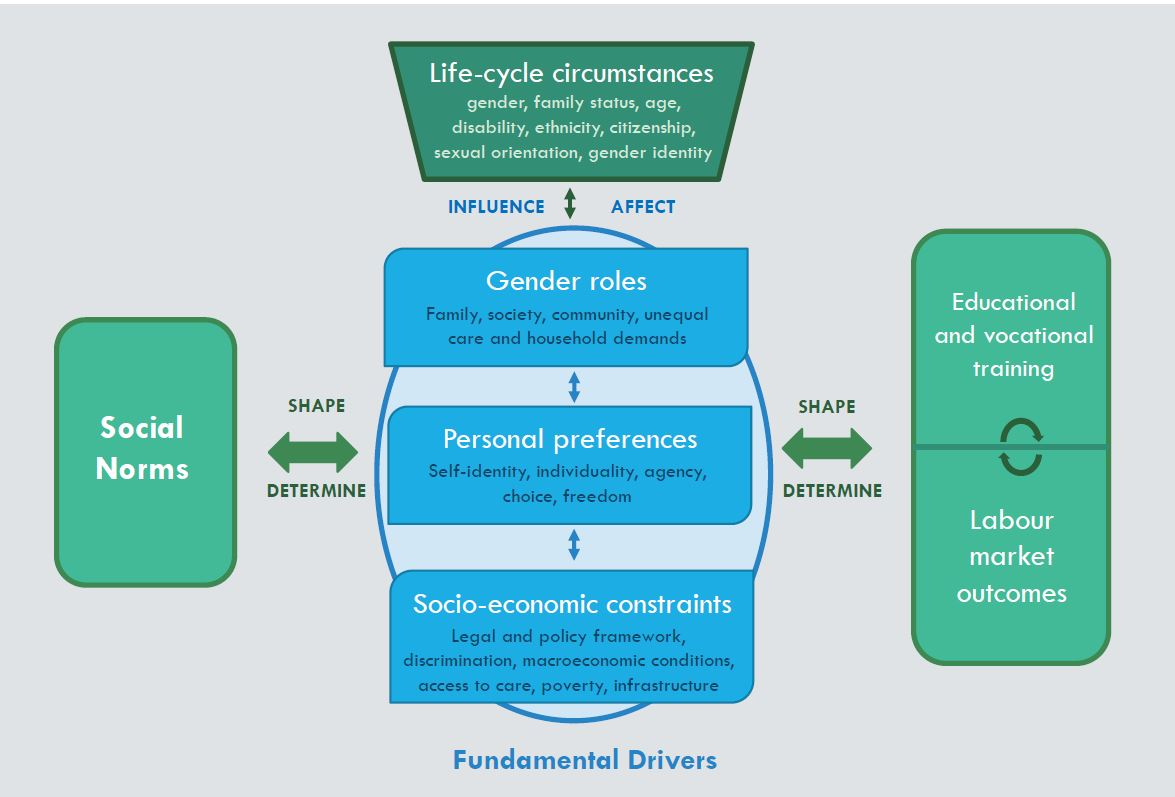
\includegraphics[width=120mm,keepaspectratio,height=0.6\textheight]{Figures/framework_1}
	\label{fig:framework}
\end{figure}

Personal preferences are an important driver of an individual's labour market outcome, within the constraints set by prevailing social norms and socio-economic factors (in conjunction with life-cycle circumstances) (figure 5). Indeed, a woman's preference for engaging in work is an expression of both what is perceived to be legitimate in her personal circumstances and her socialized identity (\cite{ilogallup2017} and Sen, 1987). In fact, many women who prefer to work, are able to choose to do so and, as result, derive pleasure and economic and social well-being from decent work opportunities. On the other hand, some women may prefer to stay at home due to a lack of jobs that are "socially acceptable" for women, because childcare costs may exceed their potential incomes or because their role within the household may be perceived as more valuable (economically and socially). However, personal preferences are also shaped by what is perceived to be legitimate and accessible, and are hence endogenous to gender norms and socio-economic constraints (\citet*{sen1995agency}).
 
Socio-economic constraints represent the institutional, economic and physical constraints faced by both men and women. As discussed above, economic conditions can dictate the availability and quality of jobs, both within and across countries. For instance, a downturn in the business cycle can temporarily provoke economic necessity within a household, in which case women often move into paid employment, so that, in effect, their labour supply acts as an insurance mechanism (Attanasio, Low and Sánchez-Marcos, 2005; Bhalotra and Umana-Aponte, 2010). Among institutional constraints, the legal and policy framework of tax systems can often impose high marginal tax rates on secondary earners with lower income, who are more likely to be women, hence disincentivizing their participation in the labour force (Stotsky, 1996; \cite{Jaumotte2003}; EC, 2015). Alternatively, the lack of care facilities poses a problem for the entire household, but in reality its effect is disproportionally felt by women due to their assigned gender role as caregivers (\cite{badgett1999assigning}). Additionally, discrimination directly creates gender gaps through the disadvantageous treatment of women in terms of payment, hiring or promotion. Importantly, since policy is, at least in part, a function of and influenced by gender social norms, it is influential in shaping the extent of socio-economic constraints and the magnitude of their effects while simultaneously reinforcing existing gender prevailing norms (Sjoberg, 2004).
  
Gender role conformity arises from traditional gender social norms that operate at multiple levels   of society, ranging from religion to economic class, race and locality. Class, patriarchy and social hierarchy, often determined by caste, ethnicity and religion, interact with one another to shape society's norms around gender roles (\cite{bardhan1984land}; \cite{klasen2012push}). As a result, women are often compelled to conform to the gender roles deemed to be acceptable by their family, community or society in order to avoid the consequences of social exclusion, insecurity or other conflicts. These attitudes towards gender roles construct a social hierarchy that not only defines women's roles in the labour market, but also adds to the disproportionate burden of household responsibilities that they must bear (Badgett and Folbre, 1999).

The three fundamental drivers as described above help determine the various labour market outcomes of women, notably (i) labour market participation, (ii) occupation or sector of employment, (iii) type of employment relationship, and (iv) income. This relationship, however, is recursive. The labour market outcomes themselves can influence the decision to participate in the labour market in the first instance. Put simply, unequal labour market outcomes (e.g. if women are paid less or have limited occupational opportunities) can shape the decision to participate. 

In addition, these labour market outcomes are interdependent. For example, if due to social norms women can only find employment in certain types of occupations that are characterized by part-time employment relationships and lead, in turn, to a wage penalty, then occupation, employment type and income are reinforcing one another.

Related is the importance of education. Educational opportunities (including access and quality) are affected by social norms. Indeed, gender differences in most developed countries can manifest themselves in the choice of study and in developing and emerging countries the level of education that is achievable (EC, 2009). In this respect, education, including vocational training, is a primary determinant of labour market outcomes. Moreover, educational attainment and the field of study determine not only labour market entry but also career trajectories (then affect other aspects of the labour market such as occupational choice and income). 

As evidenced by the discussion, there is a considerable level of inter-connectivity and inter-dependence among the drivers and labour market outcomes. With this in mind, the next section identifies and isolates - to the extent possible - the impact of these individual drivers on female labour force participation rates. The approach therefore links to the  "capabilities approach"  by capturing the voices of women expressing the challenges they face within the labour market, their preferences in terms of work, their perception of their own futures and the normative constraints on their agency which they face. Hence, this analysis strives to capture the empowerment, agency and ability of women to make decisions, both within the home and in the labour market.
